\section{System Overview and KG Design}
\label{section:overview_and_kg_design}

\subsection{Overview}
\label{section:overview}

Figure \ref{figure:overview} demonstrates an overview of our entire knowledge graph-assisted LLM post-training system. The first step is to extract the key concepts from legal cases (from U.S. jurisdictions) by utilizing an LLM and a prompt (Appendix \ref{section:appendix_prompt_kg}) that includes the KG schema (Section \ref{section:kg_design}). Then, we produce training data for both Supervised Fine-Tuning (SFT) and Preference Training. During data generation, in addition to prompts, we also employed an LLM for explanation generation (Section \ref{section:rules_sft}) and as an LLM Judge (Section \ref{section:rules_dpo}).
\begin{figure}[ht]
  \center
  
\includegraphics[width=0.5\columnwidth]{figure/overview.pdf}
  \caption{System overview.}
  \label{figure:overview}
\end{figure}

\subsection{Knowledge Graph Design}
\label{section:kg_design}

Different from prior works that extract specific entity names (e.g., Person, Company, Location, etc.), our KG focuses on extracting the key legal concepts (such as Facts and Legal Issues) in order to facilitate legal reasoning. Figure \ref{figure:kg_schema} shows the design of our legal KG, a key component of our proposed system, by following the IRAC framework.
\begin{figure}[ht]
  \center
  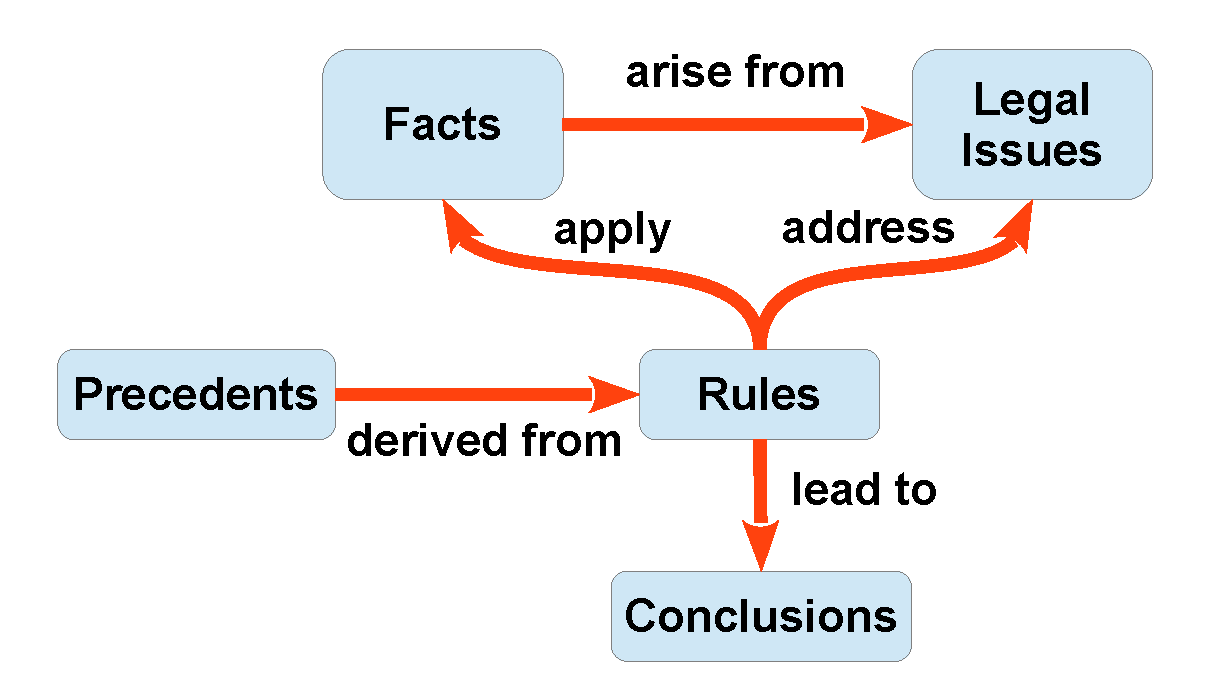
\includegraphics[width=0.5\columnwidth]{figure/kg_schema.pdf}
  \caption{Schema of our IRAC legal knowledge graph.}
  \label{figure:kg_schema}
\end{figure}

\begin{figure*}[t]
  \center
  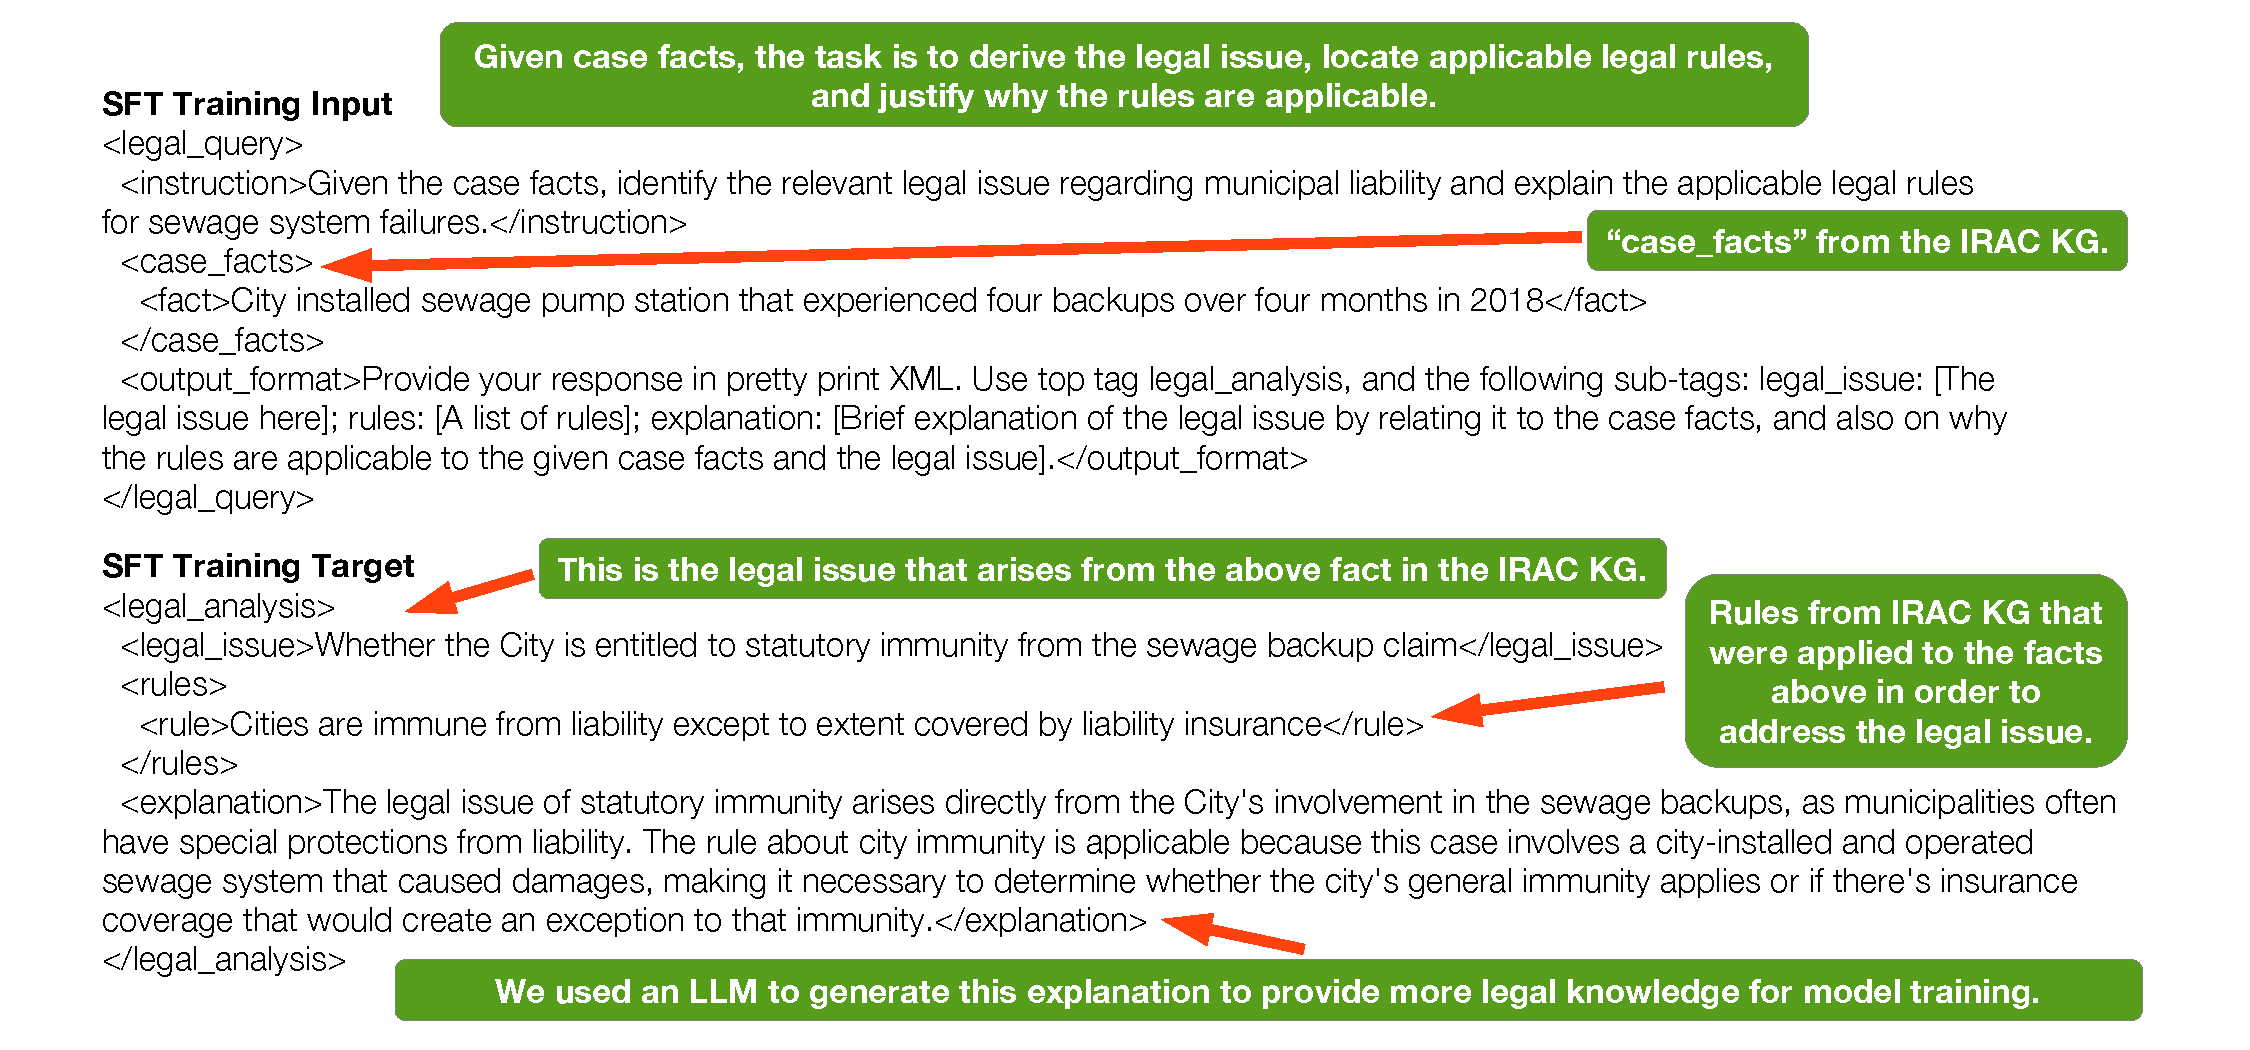
\includegraphics[width=1.0\linewidth]{figure/rules_sft.pdf}
  \caption{An example of the Rules SFT dataset.}
  \label{figure:rules_sft}
\end{figure*}

IRAC is commonly adopted for conducting legal analysis \cite{Burton2017ThinkLikeALawyer}. Even though there are variations, such as ILAC (Issue, Law, Analysis, Conclusion), IRAACP (Issue, Rule, Apply, Apply, Conclusion, Policy), etc., the core idea of legal reasoning centers around the same main concepts, i.e., Issue, Rule, Analysis and Conclusion. We consulted four legal experts on the design in order to capture the core of the legal reasoning process. Our IRAC KG includes the following components:
\begin{itemize}
  \item Legal Issues (\textbf{I}): This represents legal issues that the different parties (e.g., plaintiffs, defendants, judges, attorneys, etc.) are addressing in a legal case. Facts are things that actually happened, and the reason we have a legal case is due to the facts. Therefore, we have \textit{Legal Issues} \textbf{arise from} \textit{Facts} in our schema.
  \item Rules (\textbf{R}): This refers to legal rules. In the legal domain, prior cases (also known as precedents) that are sufficiently representative become rules that courts will reference to decide on future cases. Therefore, \textit{Rules} are \textbf{derived from} \textit{Precedents}.
  \item Analysis or Application (\textbf{A}): This denotes the legal reasoning process. When deciding on a legal case, courts will \textbf{apply} \textit{Rules} to \textit{Facts} in order to \textbf{address} the \textit{Legal Issues}.
  \item Conclusions (\textbf{C}): The analysis that courts carry out will eventually \textbf{lead to} certain \textit{Conclusions}. These are courts' rulings on the case.
\end{itemize}
